\documentclass[10pt, unicode]{beamer}
\usepackage[english]{babel}
\usepackage[utf8x]{inputenc}
\usepackage[T1]{fontenc}
\usepackage{bbding}
\usepackage{animate}
\usepackage{xcolor}
\usepackage{color}
\usepackage{colortbl}


\usepackage{numprint}
\npthousandsep{\,}
\newcommand{\quotes}[1]{``#1''}
\usetheme{Berlin}
\usecolortheme{beaver}

%title page
\title{Optimization and Applications of Deep Learning algorithms for Super Resolution in MRI}
\author{Mattia Ceccarelli}
\institute{Master Degree in Physics \\ Alma Mater Studiorum - University of Bologna}
\date{A.Y. 2019-2020}

\begin{document}

\begin{frame}
 \maketitle
 
  {\bf Supervisor}:  Prof. Gastone Castellani
 
  {\bf Co-Supervisor}: Dott. Nico Curti

\end{frame}

\begin{frame}{Single Image Super Resolution}{What is Super Resolution?}

  \setbeamercolor{block title example}{fg=black, bg=green!40!white}
  \setbeamercolor{block body example}{fg=black, bg=green!20!white}
  
  Super Resolution:
  \begin{itemize}
    \item {\bf Microscopy} -> diffraction limit
    \item {\bf Softwares}  -> enhance digital spatial resolution
  \end{itemize}

  \setbeamertemplate{itemize items}[ball]

  \begin{exampleblock}{Standard procedure}
    \begin{itemize}

      \item {\bf prior-known} High Resolution (HR) image;
      \item {\bf down-sample} for Low Resolution (LR) counterpart;
      \item Feed a Neural Network with {\bf LR images}.

    \end{itemize}
  \end{exampleblock}

\end{frame}

\begin{frame}{Deep Learning}{What is a Neural Network}

  \begin{itemize}
    \item Neural Network is a \textbf{series of non-linear multi-parametric functions}.
  \end{itemize}

  \begin{figure}[hbp]
    \centering
    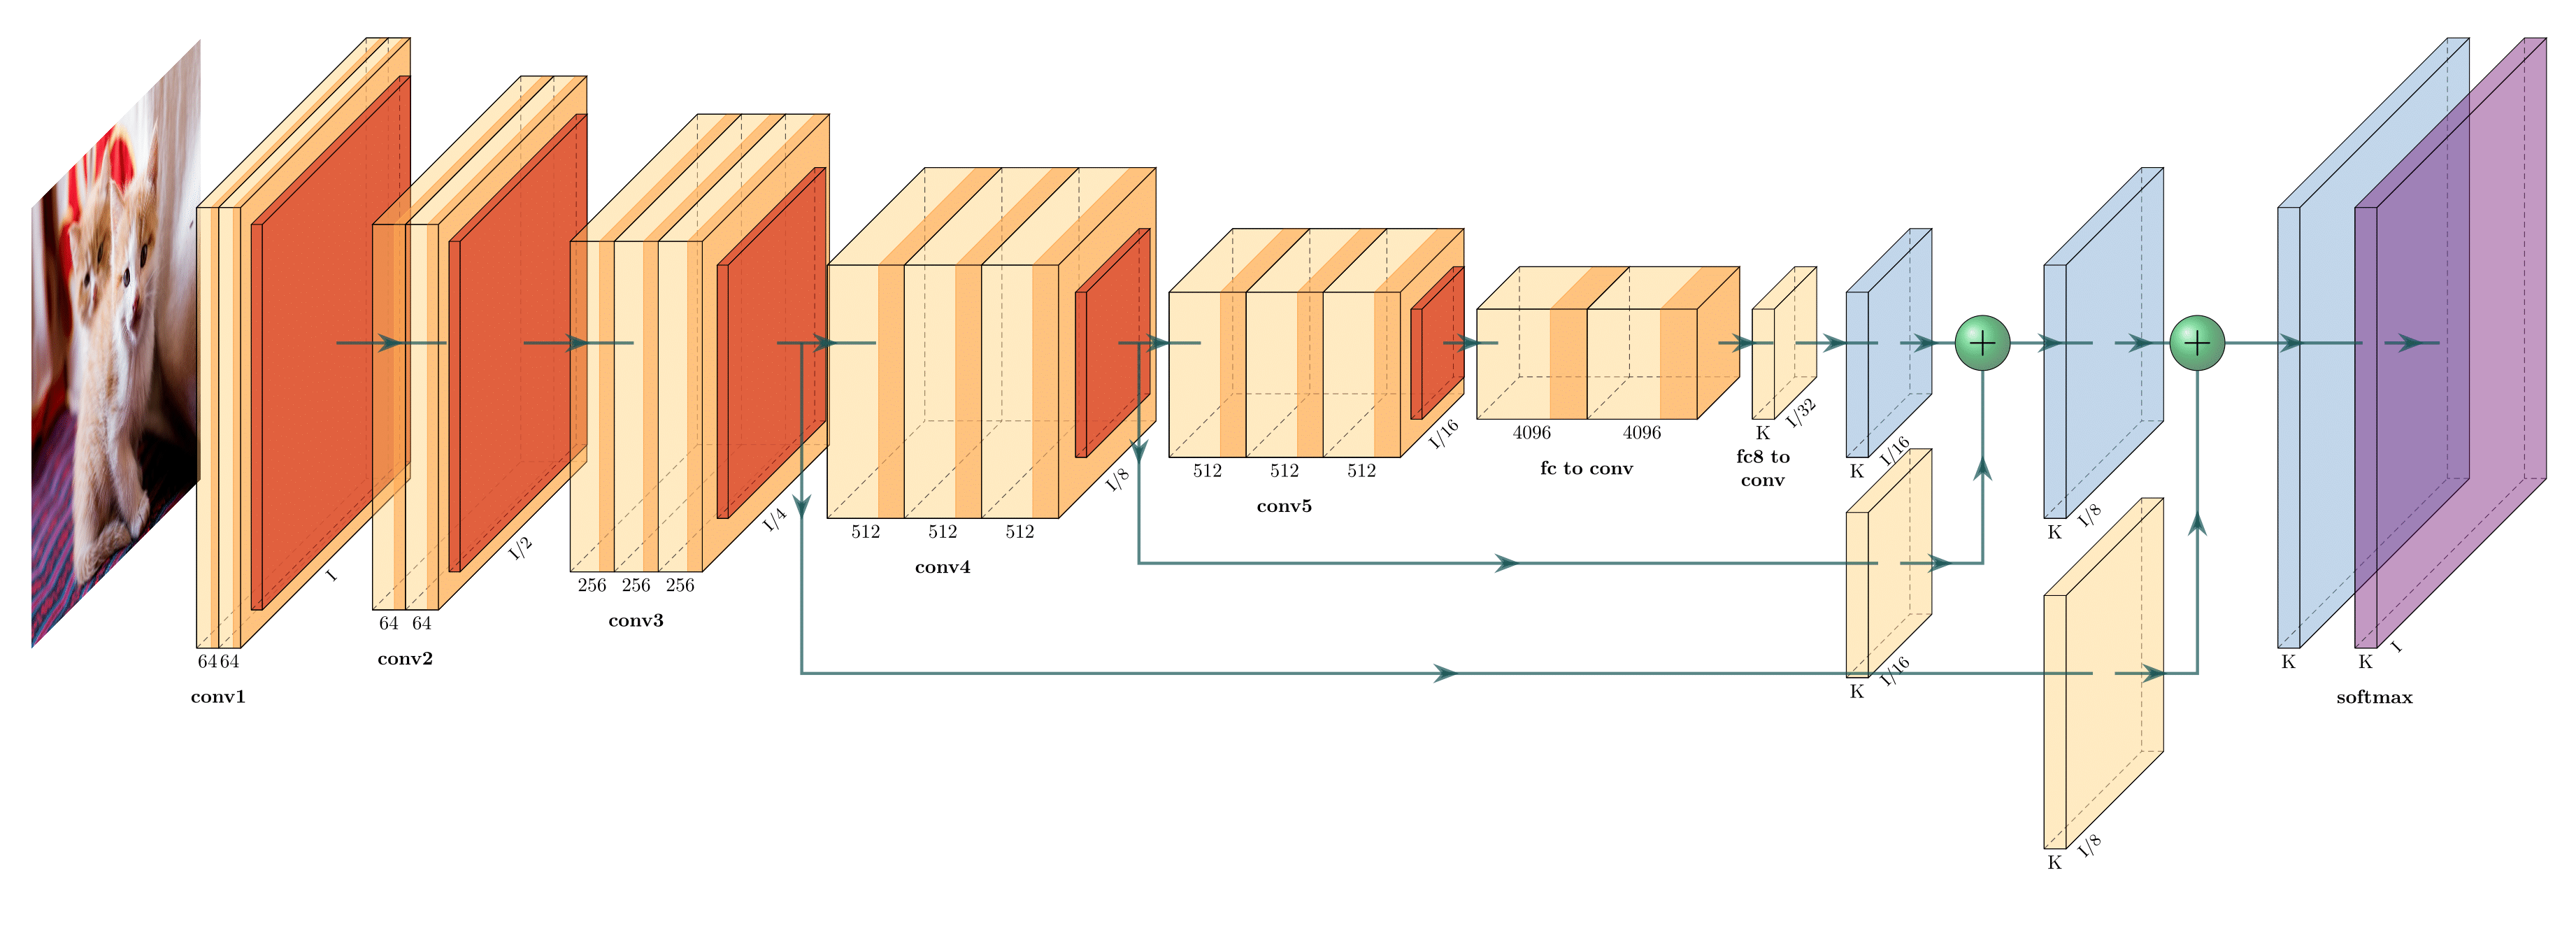
\includegraphics[width=0.85\textwidth, height=0.29\textwidth]{images/net_scheme.png}
  \end{figure}
  
  \begin{itemize}
   \item Training by \textbf{examples}
   \item Super Resolution is an \textbf{image-to-image} process
  \end{itemize}

\end{frame}

% \begin{frame}{Deep Learning}{Neural Network models}
%   
%   \begin{itemize}
%     \item The supervised training of neural network happens by feeding the model 
%           with labeled example, that are couples of inputs and expected outputs.
%     \item Then, the output is compared with the label by means of a \textbf{cost function}, which is a measure of the error made by the network.
%           
%           The objective is to modify the \textbf{parameters} of the model to minimize the cost function.
%     
%     \item {Commonly, we think about Neural Network models as tools to \textbf{reduce} problems dimensionality, i.e. starting from high-dimensional data (e.g $w\times h\times c$ image) the model predicts a class (single number)}.
% 
%     \item {In Super Resolution we have no classes but the desired output is also an image.
%           Single Image Super Resolution tasks start from an image and the aim is to reconstruct its HR counterpart.}
%   \end{itemize}
%   
%   \setbeamertemplate{itemize items}[ball]
% 
%   %\begin{block}{Objectives}
%    % \begin{itemize}
% 
%     %  \item Optimization and extension of state-of-art Neural Network libraries;
% 
%      % \item  Development of two novel libraries, for education and analytic purposes, respectively;
% 
%       %\item Improve parallelization strategies to reach the best computational performances in cluster machine without GPUs supports;
% 
%    % \end{itemize}
% 
%   %\end{block}
% 
%   %\begin{alertblock}{}
%    % All the algorithm and codes developed are \textbf{tested}, \textbf{documented} and \textbf{public available}!
% 
%     %\quad
% 
%     %\textbf{Reference:} \url{https://nico-curti2.gitbook.io/phd-thesis} (GitBook documentation).
%   %\end{alertblock}
% 
% \end{frame}
 

% \begin{frame}{State-of-art libraries}{Why another library?}
% 
%  % \scriptsize{A wide range of documentations and implementations have been written on Deep Learning and it is more and more hard to move around the different sources.}
% 
%   \scriptsize{Leaders on this topic are the multiple open-source Python libraries available on-line as \href{http://tensorflow.org}{Tensorflow}, \href{http://pytorch.org}{Pytorch} and \href{http://doi.acm.org/10.1145/2647868.2654889}{Caffe}.}
% 
%   \begin{columns}
% 
%     \begin{column}{0.5\textwidth}
% 
%       \begin{block}{Pros}
%         \begin{itemize}
%           \item[$\diamond$] Simplicity in writing complex models in a minimum number of code lines;
%           \item[$\diamond$] Simplicity of the \textsf{Python} language;
%           \item[$\diamond$] Extremely efficient in GPU environments;
%         \end{itemize}
%       \end{block}
%     \end{column}
%     \begin{column}{0.5\textwidth}
% 
%       \begin{alertblock}{Cons}
%         \begin{itemize}
%           \item[$\diamond$] Steep learning curve for complex applications or algorithm modifications;
%           \item[$\diamond$] They are not designed for CPU performances;
%         \end{itemize}
%       \end{alertblock}
%     \end{column}
% 
%   \end{columns}
% 
%   \vspace{0.5cm}
% 
%   \scriptsize{Only a small part of the research community uses deeper implementation in \textsf{C++} or other low-level programming languages.}
%   \scriptsize{About them it should be mentioned the \textsf{darknet project} of Redmon J. et al. which created a sort of standard in object detection applications using a pure \textsf{Ansi-C} library.}
% 
% \end{frame}

\begin{frame}{Developed Frameworks}{Byron and NumPyNet}
%  \scriptsize
 
  \setbeamercolor{block title alerted}{fg=black, bg=blue!40!white}
  \setbeamercolor{block body alerted}{fg=black, bg=blue!20!white}

  \setbeamertemplate{itemize/enumerate body begin}{}
  \setbeamertemplate{itemize/enumerate subbody begin}{}

    \begin{alertblock}{NumPyNet \hfill
\includegraphics[width=0.03\textwidth]{images/python.png}}
    \begin{itemize}
      \item Readable and Simple \textbf{\textsf{Python}} code. 

      \item Overcomes the common ``\textbf{black-box}'' idea of Neural Network 
      
      \item \textbf{Test} optimized code, \textbf{Experiment} with models and \textbf{Learn} 

    \end{itemize}
  \end{alertblock} 
 
  \setbeamercolor{block title alerted}{fg=black, bg=orange!40!white}
  \setbeamercolor{block body alerted}{fg=black, bg=orange!20!white}

  \setbeamertemplate{itemize/enumerate body begin}{}
  \setbeamertemplate{itemize/enumerate subbody begin}{}

  \begin{alertblock}{Byron \hfill
\includegraphics[width=0.03\textwidth]{images/cpp.png}}
    \begin{itemize}
      \item Efficiency and flexibility of \textbf{\textsf{C++}} 

      \item \textbf{Optimized for image processing}, common in biomedical research
      
      \item Tailored around \textbf{CPU} usage
    
    \end{itemize}
  \end{alertblock}
  
  %\vfill\scriptsize{* The library was developed in collaboration with Dott. Baroncini.}

\end{frame}


% \begin{frame}{Standard up/down scaling algorithms}{Single Image Super Resolution}
% 
%   \setbeamertemplate{itemize items}[ball]
% 
%   \begin{columns}
%     \begin{column}{0.4\textwidth}
%       \scriptsize{Interpolation algorithms:}
%       \begin{itemize}
%         \item \textbf{Nearest};
%         \item \textbf{Bicubic};
%         \item \textbf{Lanczos};
%       \end{itemize}
% 
%       \scriptsize{The best compromise between computation cost and efficiency is given by the Bicubic interpolation algorithm}.
%       \scriptsize{Given a pixel, the interpolation function evaluates the 4 pixels around it applying a filter given by the equation:}
%     \end{column}
%     \begin{column}{0.6\textwidth}
%       \begin{figure}
%         \centering
%         \def\svgwidth{\textwidth}
%         \input{./up_down_sampling.pdf_tex}
%         %\caption{\tiny{Up/Down sampling with scale factor equal to 2.}}
%       \end{figure}
%     \end{column}
%   \end{columns}

%   \
%   \begin{equation*}
%   \hspace{-0.75cm}\scriptsize{
%   k(x) = \frac{1}{6} \left\{ \begin{array}{rc}
%     (12 - 9B - 6C) |x|^3 + (-18 + 12B + 6C) |x|^2 + (6 - 2B)           & \mbox{if}        |x| < 1 \\
%     (−B − 6C) |x|^3 + (6B + 30C) |x|^2 + (−12B − 48C) |x| + (8B + 24C) & \mbox{if} 1 \leq |x| < 2 \\
%     0                                                                  & \mbox{otherwise}         \\
%     \end{array}
%     \right.
%   }
%   \end{equation*}
%   \\
%   \scriptsize{where $x$ identifies each pixel below the filter.}
%   \scriptsize{Commonly values used for the filter parameters are $B=0$ and $C=0.75$ (used by \textsf{OpenCV} library) or $B=0$ and $C=0.5$ used by \textsf{Matlab}}.
% 
%   \scriptsize{\textbf{NOTE:} the nearest interpolation could be achieved also using \emph{Pooling} algorithm.}

% \end{frame}

\begin{frame}{Image Quality}{Quantitative Evaluation}

  \setbeamercolor{block title}{fg=black, bg=blue!40!white}
  \setbeamercolor{block body}{fg=black, bg=blue!20!white}

  \setbeamercolor{block title alerted}{fg=black, bg=orange!40!white}
  \setbeamercolor{block body alerted}{fg=black, bg=orange!20!white}

  \setbeamertemplate{itemize/enumerate body begin}{\scriptsize}
  \setbeamertemplate{itemize/enumerate subbody begin}{\scriptsize}


  \begin{columns}
    \begin{column}{0.48\textwidth}
      \hspace{-0.75cm}
      \begin{block}{PSNR - Peak Signal to Noise Ratio}
        \begin{itemize}
          \item Measure the quality of {\bf lossy} reconstructions;

          \begin{equation*}
          \hspace{-0.75cm}
          PSNR = 20 \cdot \log_{10}\left( \frac{\max(I)}{\sqrt(MSE)} \right)
          \end{equation*}
          \\
          where $MSE$ is :
          \vspace{-0.2cm}
          \begin{equation*}
            \hspace{-0.75cm}
            MSE = \frac{1}{N}\sum_{i=1}^{N} (I_i - K_i)^2
          \end{equation*}
          
        \end{itemize}
      \end{block}
    \end{column}
    \begin{column}{0.6\textwidth}
      \begin{alertblock}{SSIM - Structural SIMilarity index}
        \begin{itemize}
          \vspace{.4cm}
          \item It evaluates the structural similarity between two images taking into account {\bf visible improvements}

          \begin{equation*}
          \hspace{-0.75cm}
          SSIM(I, K) = \frac{1}{N}\sum_{i=1}^{N} \frac{(2\mu_x\mu_y + c_1)(2\sigma_{xy} + c_2)}{ ({\mu_x}^2 + {\mu_y}^2 + c_1)({\sigma_x}^2 + {\sigma_y}^2 + c_2) }
          \end{equation*}
          \vspace{.4cm}
        \end{itemize}
      \end{alertblock}

%       \begin{tabular}{lcc}
%         \hline \rowcolor{green!20!white}
%                           & \textbf{PSNR (dB)} & \textbf{SSIM ($\in [-1, 1]$)} \\
%         \hline
%         \textbf{Nearest}  & 25.118             & 0.847                         \\
%         \textbf{Bicubic}  & 27.254             & 0.894                         \\
%         \textbf{Lanczos}  & 26.566             & 0.871                         \\
%         \hline
%       \end{tabular}
    \end{column}

  \end{columns}

\end{frame}


\begin{frame}{Models}{Models Implemented and Tested in Byron}
  
  \centering
  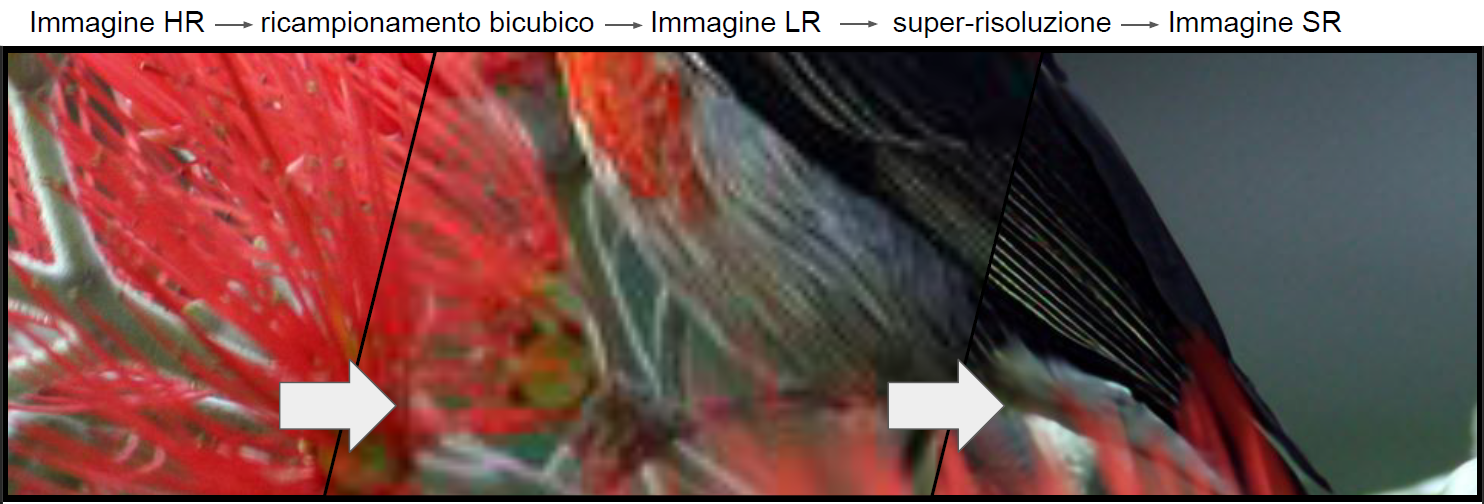
\includegraphics[width=0.78\linewidth]{images/compare.png}
  
  {Trained on \textbf{RGB Natural} images -> \textbf{Transfer Learning}}
  \begin{columns}
    \begin{column}{0.5\textwidth}
      \setbeamercolor{block title alerted}{fg=black, bg=orange!40!white}
      \setbeamercolor{block body alerted}{fg=black, bg=orange!20!white}
      \begin{alertblock}{EDSR - Enhanced Deep SR}
        \scriptsize{
        \begin{tabular}{lc}
          \hline \rowcolor{orange!20!white}
                                   & Number of    \\
          \rowcolor{orange!20!white}
          Layer                     & Parameters   \\
          \hline
          Conv. input                 & 6912          \\
          Conv. (32 residual block)   & 589824     \\
          Conv. (pre-shuffle)         & 589824        \\
          Conv. (upsample block)   & 2359296       \\
          Conv. output               & 6912        \\
          \hline
        \end{tabular}
        }
        \scriptsize{Average Time on $510\times339$ image: $576.92$~s.}
        \scriptsize{More than \textbf{40 million} parameters}
      \end{alertblock}
    \end{column}
    
    \begin{column}{0.5\textwidth}
      \setbeamercolor{block title}{fg=black, bg=blue!40!white}
      \setbeamercolor{block body}{fg=black, bg=blue!20!white}

      \begin{block}{WDSR - Wide Deep SR}
        \scriptsize{
        \begin{tabular}{lc}
          \hline \rowcolor{blue!20!white}
                                      & Number of    \\
          \rowcolor{blue!20!white}
          Layer                         & Parameters   \\
          \hline
          Conv. input 1                 & 864     \\
          Conv. 1 (32 residual block)   & 55296   \\
          Conv. 2 (32 residual block)   & 55296   \\
          Conv. (pre-shuffle)           & 13824   \\
          Conv. input 2 (pre-shuffle)   & 3600    \\
          \hline
        \end{tabular}
        }
        \scriptsize{Average Time on $510\times339$ image: $46.35$~s.}

        \scriptsize{$\sim3$ million parameters}
      \end{block}
    \end{column}
  \end{columns}

\end{frame}



% \begin{frame}{EDSR - Enhanced Deep Super Resolution}{Super Resolution Models}
%   \centering
%   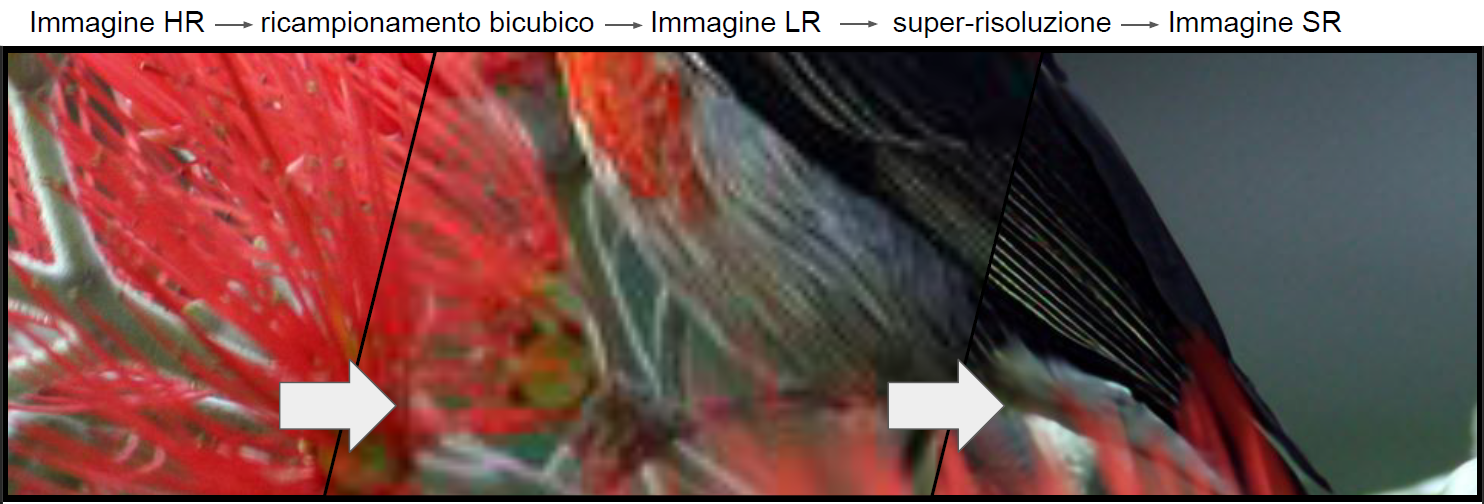
\includegraphics[width=0.78\linewidth]{images/compare.png}
% 
%   \setbeamercolor{block title alerted}{fg=black, bg=orange!40!white}
%   \setbeamercolor{block body alerted}{fg=black, bg=orange!20!white}
% 
%   \begin{alertblock}{Architecture}
%     \scriptsize{
%     \begin{tabular}{lccc}
%       \hline \rowcolor{orange!20!white}
%                                &  Channels     & Filter     & Number of    \\
%       \rowcolor{orange!20!white}
%       Layer                    & input/output  & dimensions & Parameters   \\
%       \hline
%       Conv. input              & 3/256      & $3\times3$   & 6912          \\
%       Conv. (32 residual block)   & 256/256    & $3\times3$   & 589824        \\
%       Conv. (pre-shuffle)      & 256/256    & $3\times3$   & 589824        \\
%       Conv. (upsample block)   & 256/1024   & $3\times3$   & 2359296       \\
%       Conv. output             & 256/3      & $3\times3$   & 6912          \\
%       \hline
%     \end{tabular}
%     }
% 
%     \vspace{0.5cm}
%     \scriptsize{Average Time on $510\times339$ image: $576.92$~s.}
% 
%     \scriptsize{Winner of the \textbf{NTIRE 2017}. More than \textbf{40 million} of parameters}
%   \end{alertblock}
% 
% \end{frame}
% 
% \begin{frame}{WDSR - Wide Deep Super Resolution}{Super Resolution Models}
%   \centering
%   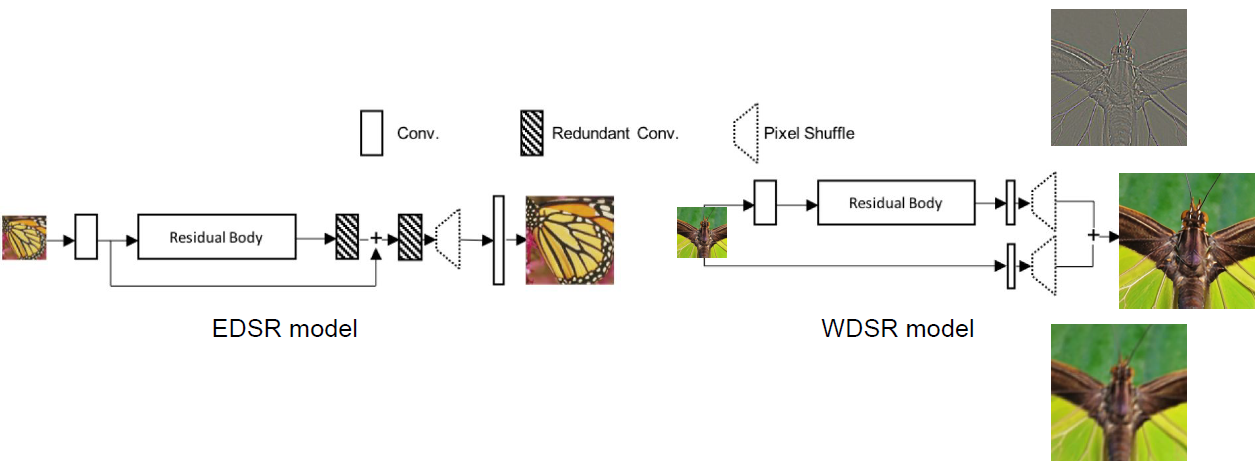
\includegraphics[width=0.7\linewidth]{images/SR_models.png}
% 
%   \setbeamercolor{block title}{fg=black, bg=blue!40!white}
%   \setbeamercolor{block body}{fg=black, bg=blue!20!white}
% 
%   \begin{block}{Architecture}
%     \scriptsize{
%     \begin{tabular}{lccc}
%       \hline \rowcolor{blue!20!white}
%                                   &  Channels     & Filter     & Number of    \\
%       \rowcolor{blue!20!white}
%       Layer                       & input/output  & dimensions & Parameters   \\
%       \hline
%       Conv. input 1               & 3/32       & $3\times3$   & 864     \\
%       Conv. 1 (32 residual block)    & 32/192     & $3\times3$   & 55296   \\
%       Conv. 2 (32 residual block)    & 192/32     & $3\times3$   & 55296   \\
%       Conv. (pre-shuffle)         & 32/48      & $3\times3$   & 13824   \\
%       Conv. input 2 (pre-shuffle) & 3/48       & $5\times5$   & 3600    \\
%       \hline
%     \end{tabular}
%     }
% 
%     \vspace{0.5cm}
%     \scriptsize{Average Time on $510\times339$ image: $46.35$~s.}
% 
%     \scriptsize{Winner of the \textbf{NTIRE 2018}. $\sim3$ million of parameters, \textbf{less than $10\%$ of EDSR model}!}
%   \end{block}
% 
% \end{frame}

\begin{frame}{Dataset}{MRI pre-processing description}
  
  \begin{columns}
    
    \begin{column}{0.5\textwidth}
      \vspace{-0.5cm}
      \begin{figure}
        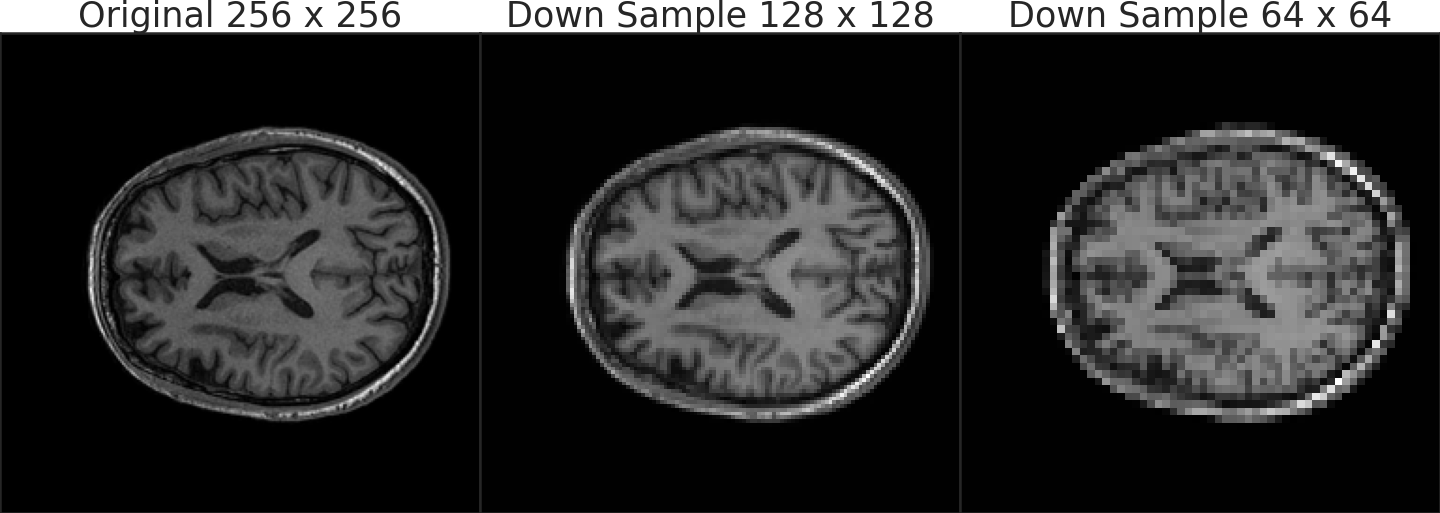
\includegraphics[scale=0.13]{./images/donwsamples.png}
        \caption{T1-weighted downsamplings}
      \end{figure}
      \begin{figure}
        \vspace{-1cm}
        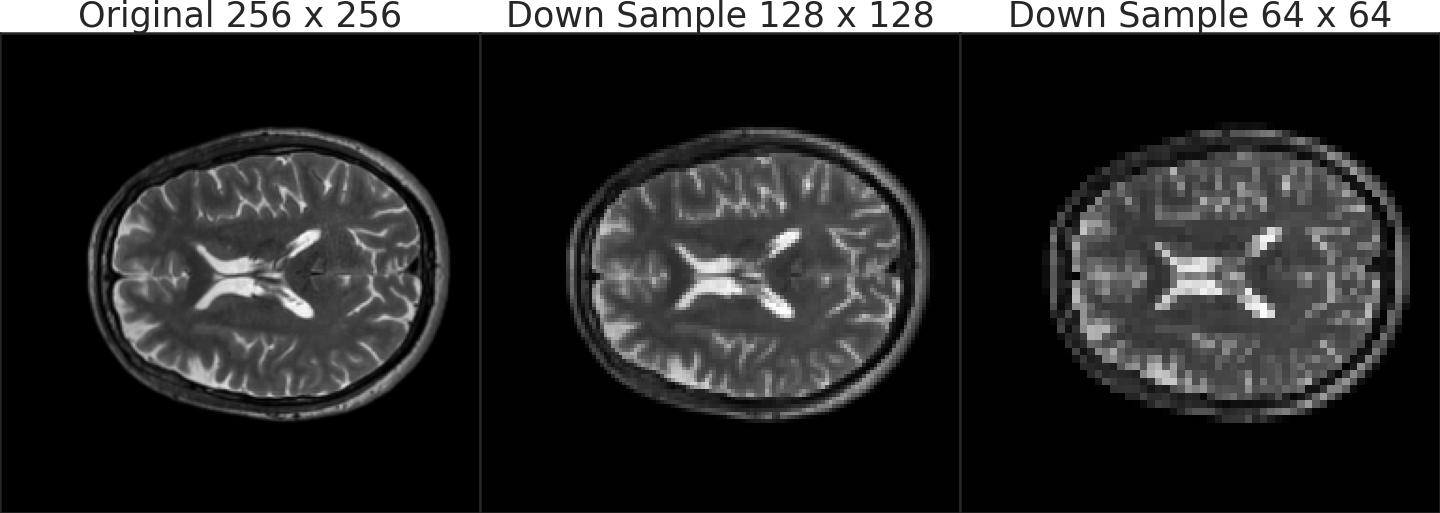
\includegraphics[scale=0.13]{./images/donwsamples_t2.png}
        \caption{T2-weighted downsamplings}
      \end{figure}
    \end{column}

    \begin{column}{0.4\textwidth}
      \vspace{-1.5cm}
      \begin{itemize}
        \item Public NAMIC dataset of 5 patients -> originals HR
        \item Gaussian blurring
        \item Donwscaling (x2 and x4)
        \item Re-upsamples with NN and Bicubic Algorithm (BC)
      \end{itemize}
    \end{column}
  
  \end{columns}

\end{frame}

% \begin{frame}{Dataset}{MRI re-usampling}
% 
%   \begin{itemize}
%     \item 20 input rotations for LR images  
%     \item The LR images are processed by the models
%     \item The up-scaled slices are compared with the originals with PSNR and SSIM.
%   \end{itemize}
% 
%   \begin{figure}
%     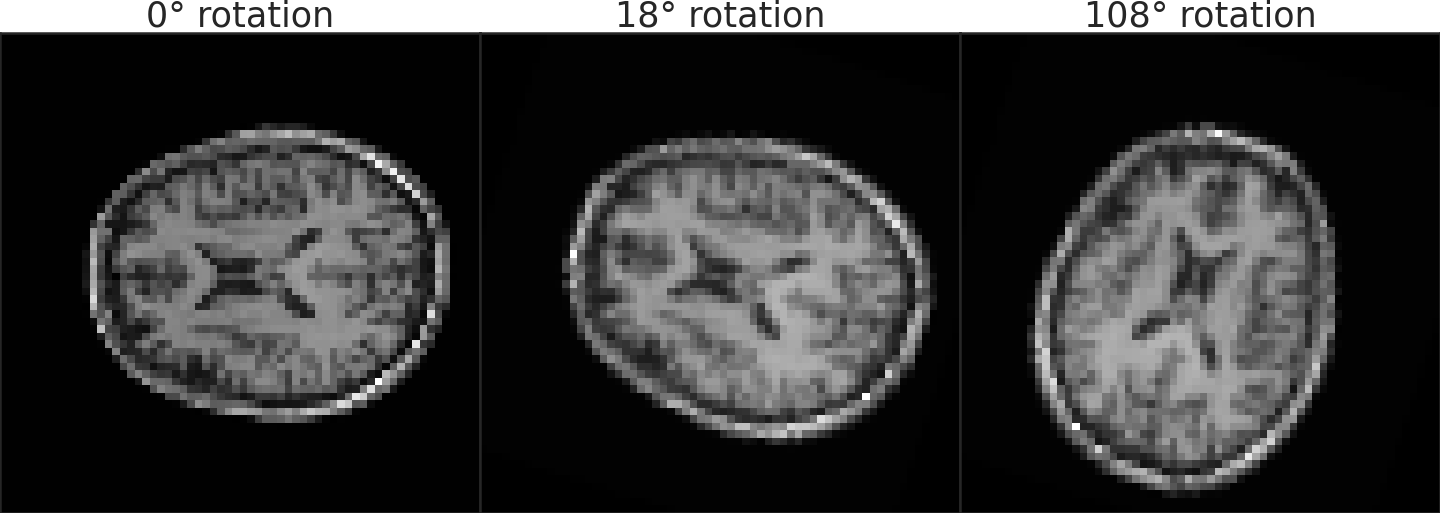
\includegraphics[scale=0.19]{./images/rotations_aligned.png}
%   \end{figure}
% 
% \end{frame}

% Results.

\begin{frame}{Upsample Comparisons}{EDSR and Bicubic x2}
  \small
    \begin{columns}
    \begin{column}{0.5\textwidth}
      T1-weighted: 
      \begin{itemize}
        \item Mean trends on patient and angles.
        \item SR scores are higher than BC counterparts
        \item The three RGB channels perfoms differently
      \end{itemize}
      \begin{figure}
        \vspace{-0.3cm}
        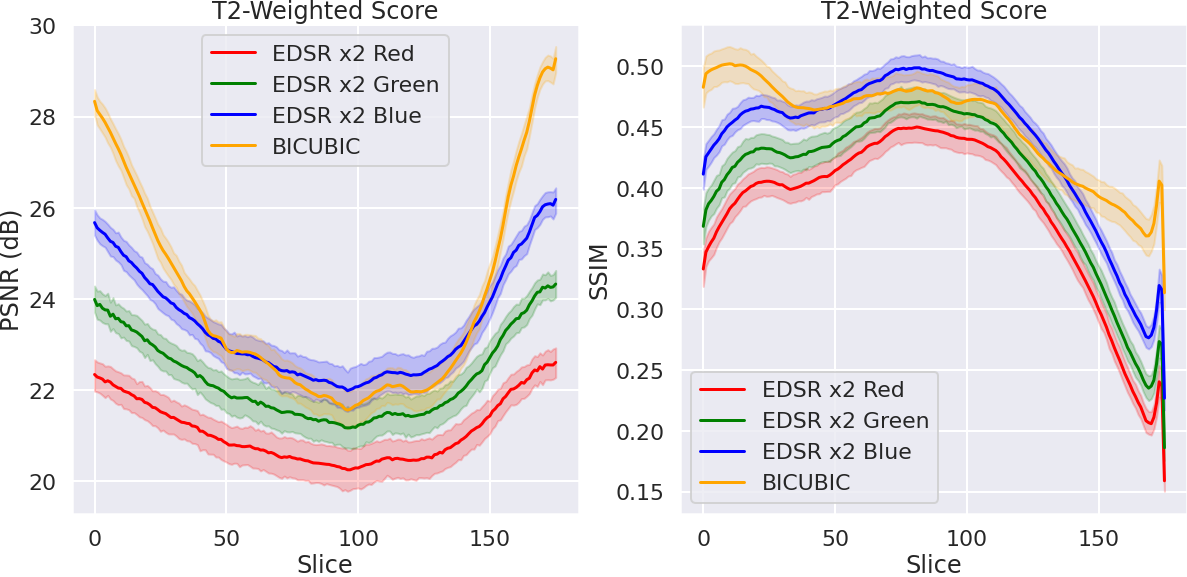
\includegraphics[scale=0.14]{./images/EDSR_score_slide_t2_all.png}
      \end{figure}
    \end{column}

    \begin{column}{0.5\textwidth}
      \begin{figure}
        \vspace{-1.6cm}
        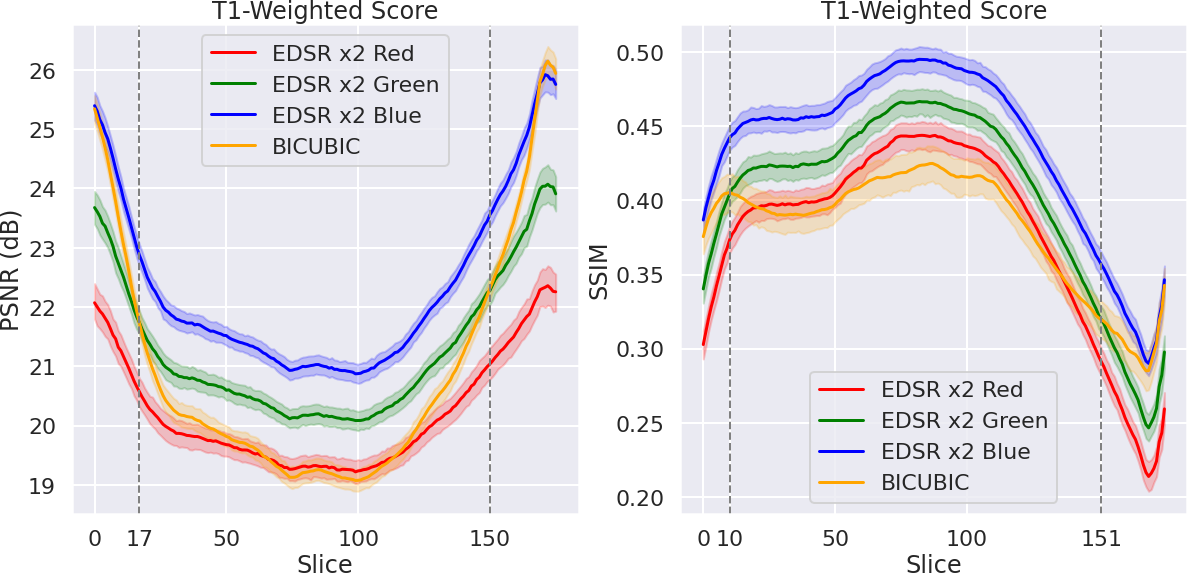
\includegraphics[scale=0.14]{./images/EDSR_score_slide_t1_all.png} 
      \end{figure}
      \vspace{0.3cm}
      T2-weighted:
      \begin{itemize}
        \item RGB channels still have different performances 
        \item BC and SR are comparable on most informative parts
      \end{itemize}

    \end{column}
  \end{columns}  

%   \begin{figure}
%     \centering
%     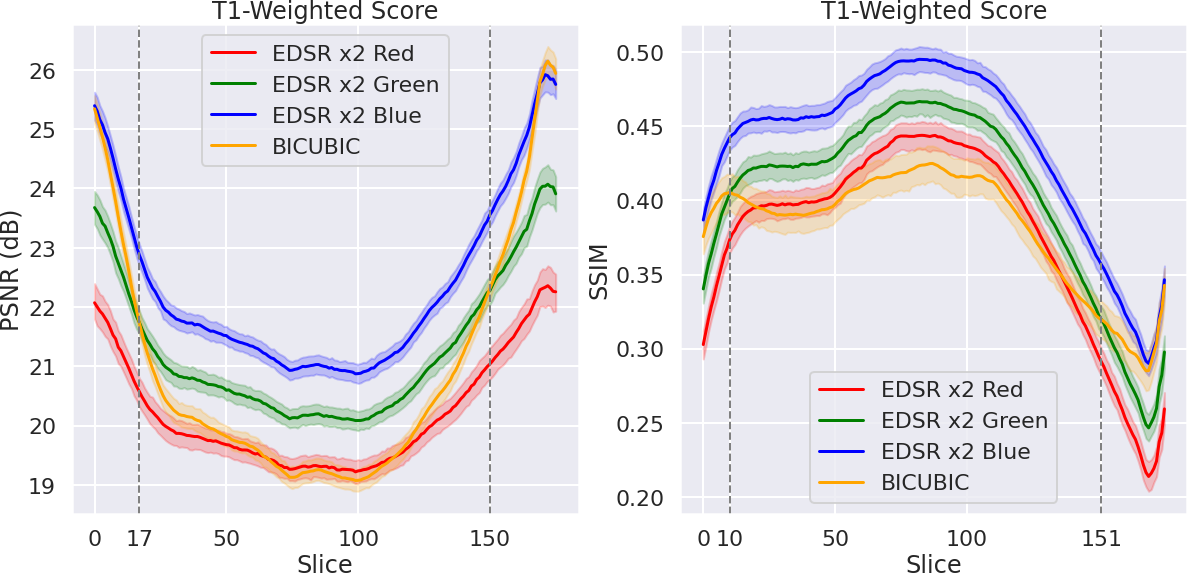
\includegraphics[scale=0.21]{./images/EDSR_score_slide_t1_all.png}
%     \caption{\scriptsize Average trends of PSNR (left) and SSIM (right) for the three channels (Red, Blue, Green lines) of the Super Resolution EDSR model compared with the bicubic algorithm scores (Yellow) as functions of the slices. The average is performed for every patients and for every rotation,  cosidering only T1 weighted NMR. The dotted lines highlights the slices where the bicubic and super-resolution green channel performances intersect.}
%     \end{figure}
\end{frame}

\begin{frame}{Upsample Comparisons}{WDSR and Bicubic x4}

  \begin{columns}
    
    \begin{column}{0.5\textwidth}
      \begin{figure}
        \vspace{-1cm}
        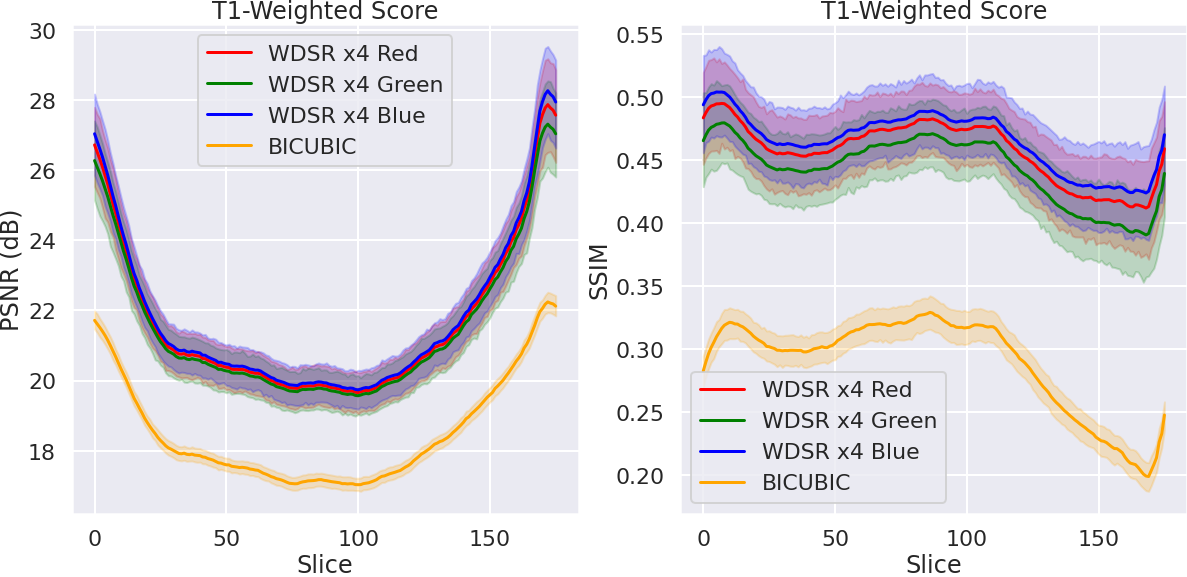
\includegraphics[scale=0.14]{./images/WDSR_score_slide_t1_all.png} 
        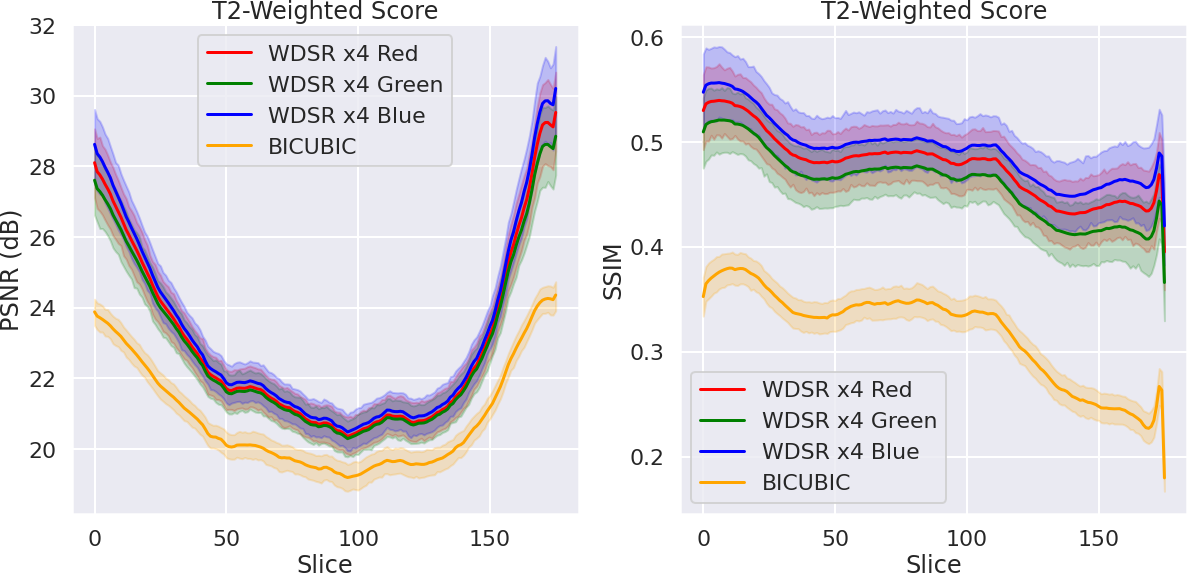
\includegraphics[scale=0.14]{./images/WDSR_score_slide_t2_all.png}
      \end{figure}
    \end{column}
    
    \begin{column}{0.5\textwidth}
      \begin{itemize}
        \item Much less variance between channels
        \item Both SSIM and PSNR shows better performances
      \end{itemize}
    \end{column}
  \end{columns}  

%   \begin{figure}
%     \centering
%     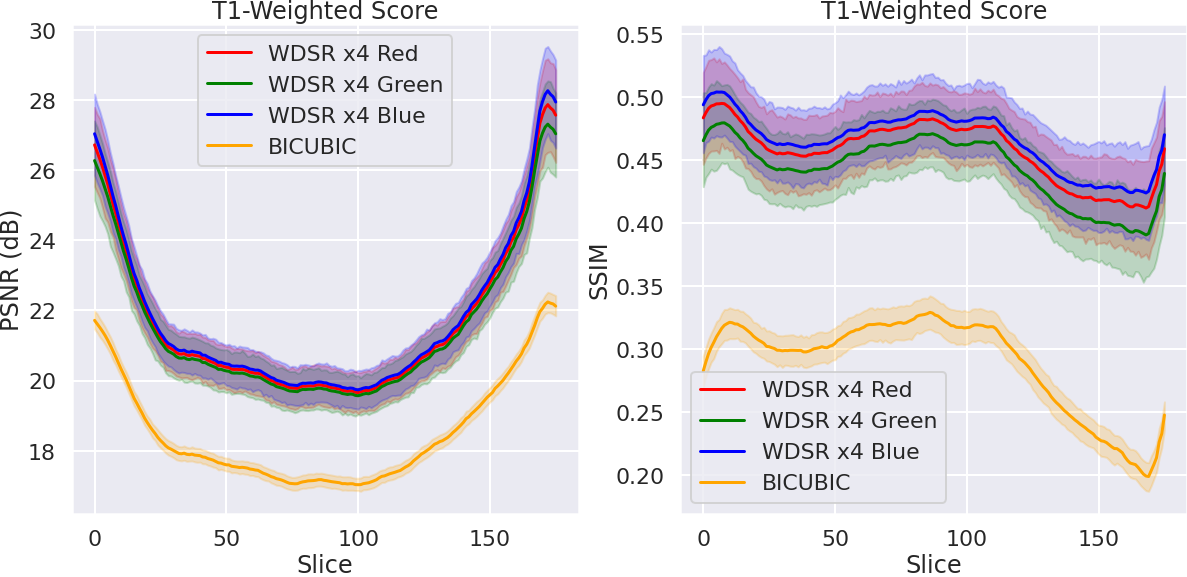
\includegraphics[scale=0.21]{./images/WDSR_score_slide_t1_all.png}
%     \caption{\scriptsize Average trends of PSNR (left) and SSIM (right) for the three channels (Red, Blue, Green lines) of the Super Resolution WDSR model compared with the bicubic algorithm scores (Yellow) as functions of the slices. The average is performed for every patients and for every rotation, for T1-weighted NMRs.}
%   \end{figure}
 
\end{frame}


\begin{frame}{Error Localization}{EDSR and Bicubic x2}

  \begin{figure}
    \centering
    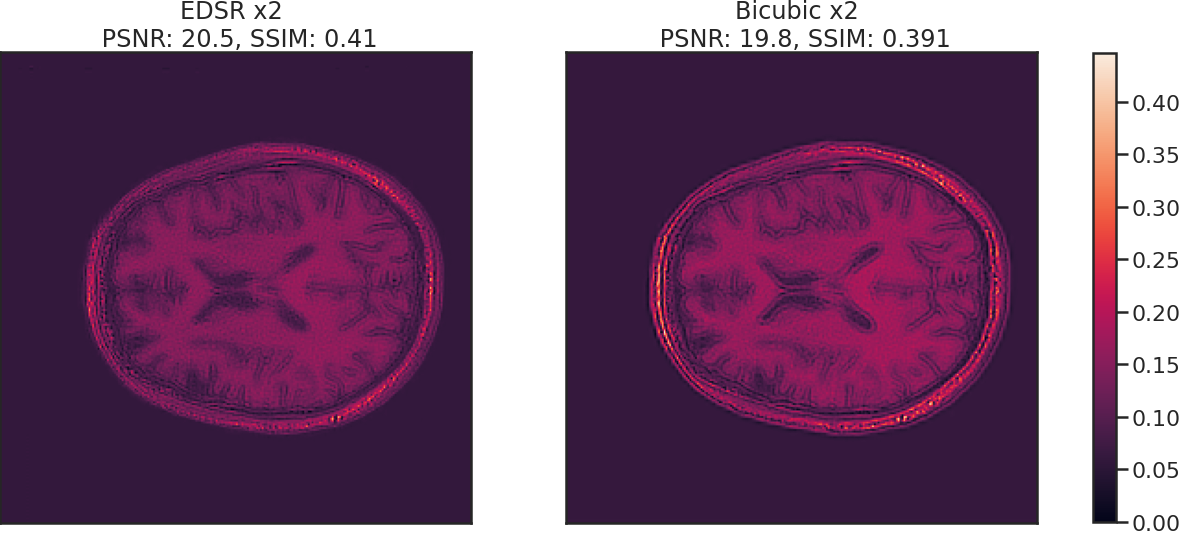
\includegraphics[scale=0.2]{./images/diff-edsr.png}
  \end{figure}
  
  \begin{itemize}
   \item Pixel-wise absolute difference between reconstructions and originals
   \item Higher differences located around scalps
   \item Background $\neq$ 0
  \end{itemize}


\end{frame}

\begin{frame}{Error Localization}{EDSR and Bicubic x2 On T1-weighted patients }

  \begin{figure}
    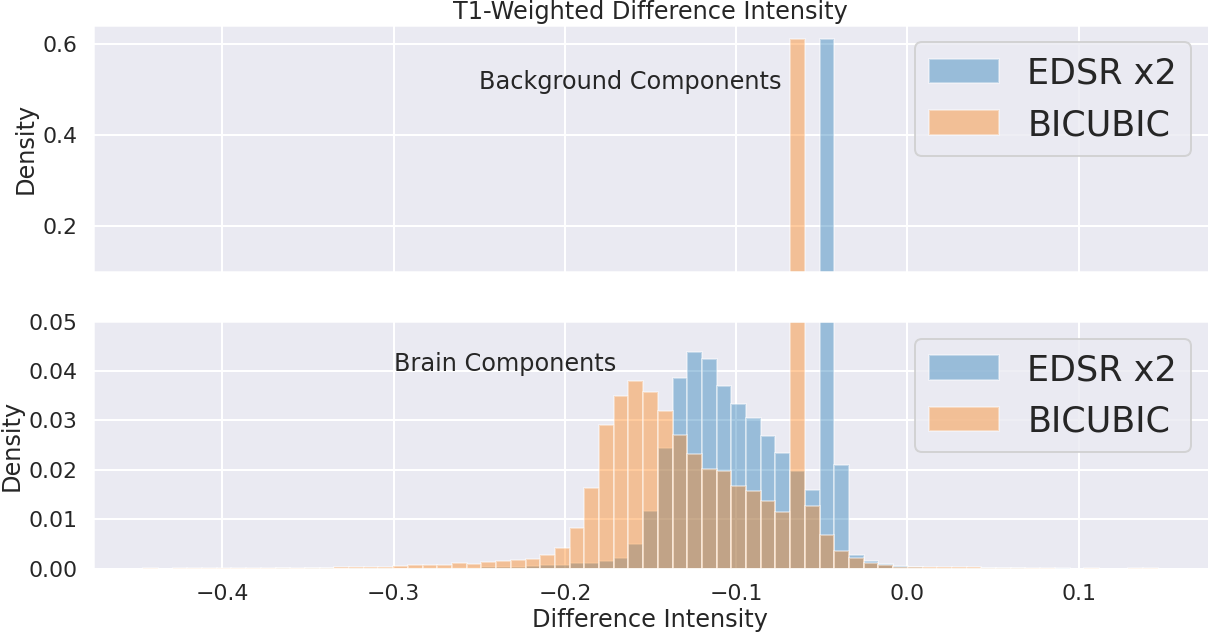
\includegraphics[scale=0.2]{./images/EDSR_diff_histo_t1.png}
  \end{figure}
  
  \begin{itemize}
    \item Clear distiction between two components
    \item Heavy background components
    \item Pixel values are  overestimated
  \end{itemize}

\end{frame}

\begin{frame}{Brain Extraction}{BET - Brain Extraction Tool}

  \begin{figure}
    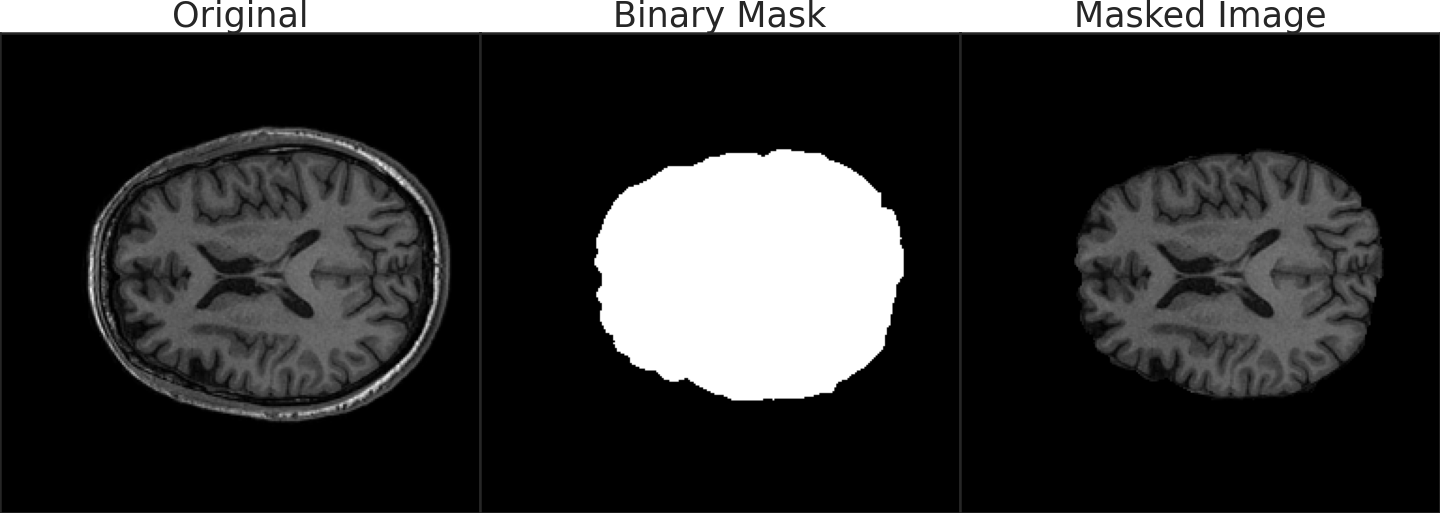
\includegraphics[scale=0.2]{./images/mask_example.png}
  \end{figure}
  
  \begin{itemize}
    \item BET is a standard tool in MRI analysis. Two approaches:
    \begin{itemize}
      \item [1.] Extract masks for originals and reconstructions and compare
      \item [2.] Use the masks obtained from HR originals to evaluate 
                 reconstructions.
    \end{itemize}
  
  \end{itemize}

\end{frame}


\begin{frame}{Brain Extraction}{BET - Masks Analysis}

  \begin{columns}
    \begin{column}{0.5\textwidth}
      \hspace{2cm}
      \begin{itemize}
        \item  Three masks from originals and reconstructions
        \item  Intersection over Union: 
      \end{itemize}
      
      \vspace{0.2cm}
      \begin{figure}
        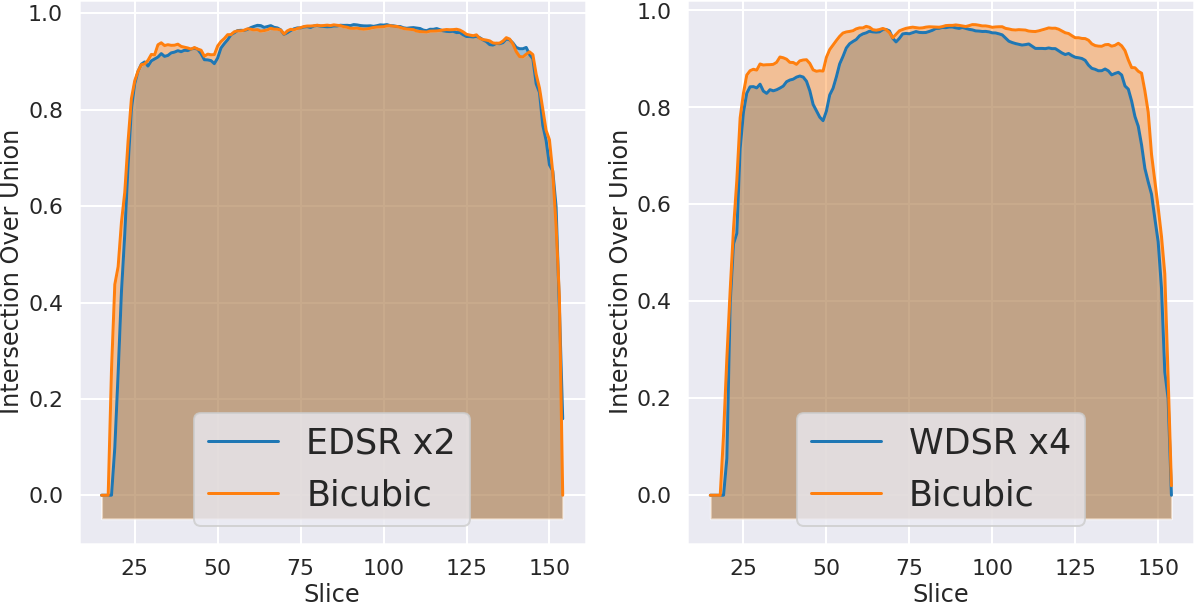
\includegraphics[scale=0.14]{./images/iou_scores.png}
      \end{figure}
    \end{column}

    \begin{column}{0.5\textwidth}
      \vspace{-1cm}
      \begin{figure}
        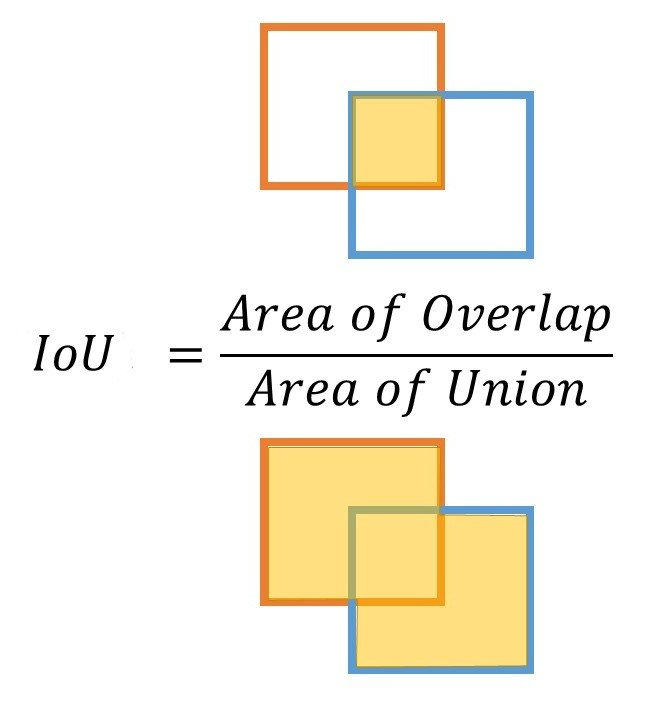
\includegraphics[scale=0.15]{./images/IoU-ex.jpg}
      \end{figure}
      \begin{itemize}
        \item IoU > 0.90
        \item EDSR comparable results
        \item WDSR not adapt for BET 
      \end{itemize}
    \end{column}
  \end{columns}
\end{frame}

\begin{frame}{Brain Extraction}{BET - Background Removal} 

  \begin{columns}
    
    \begin{column}{0.5\textwidth}
      \begin{figure}
        \vspace{-1cm}
        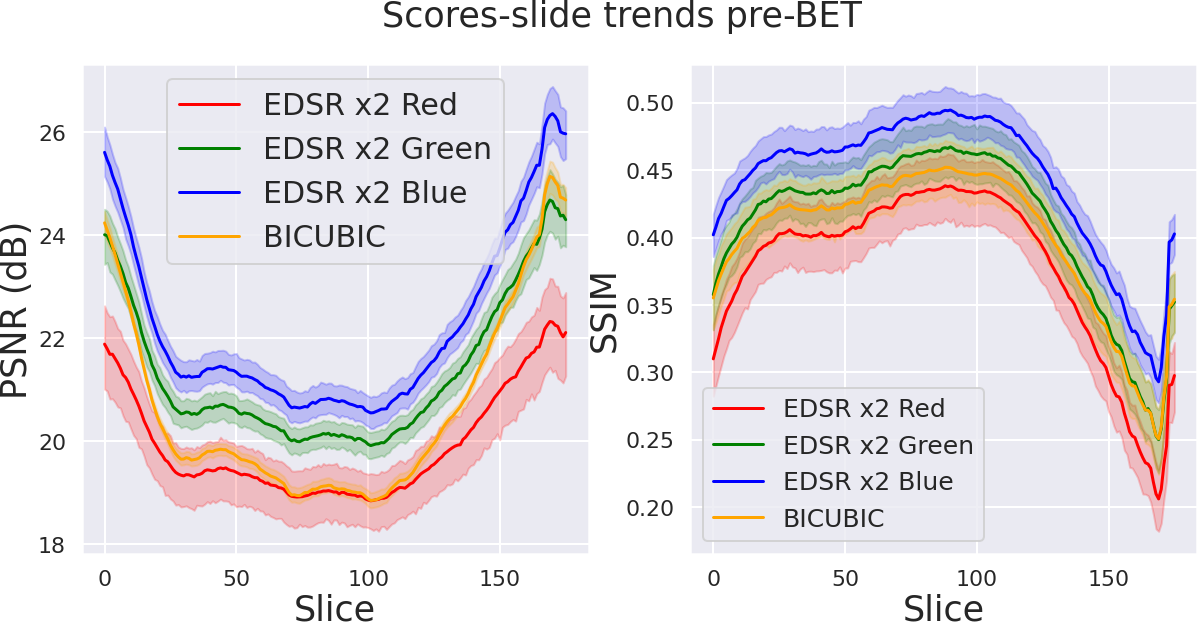
\includegraphics[scale=0.14]{./images/EDSR_score_t1_prebet.png} 
        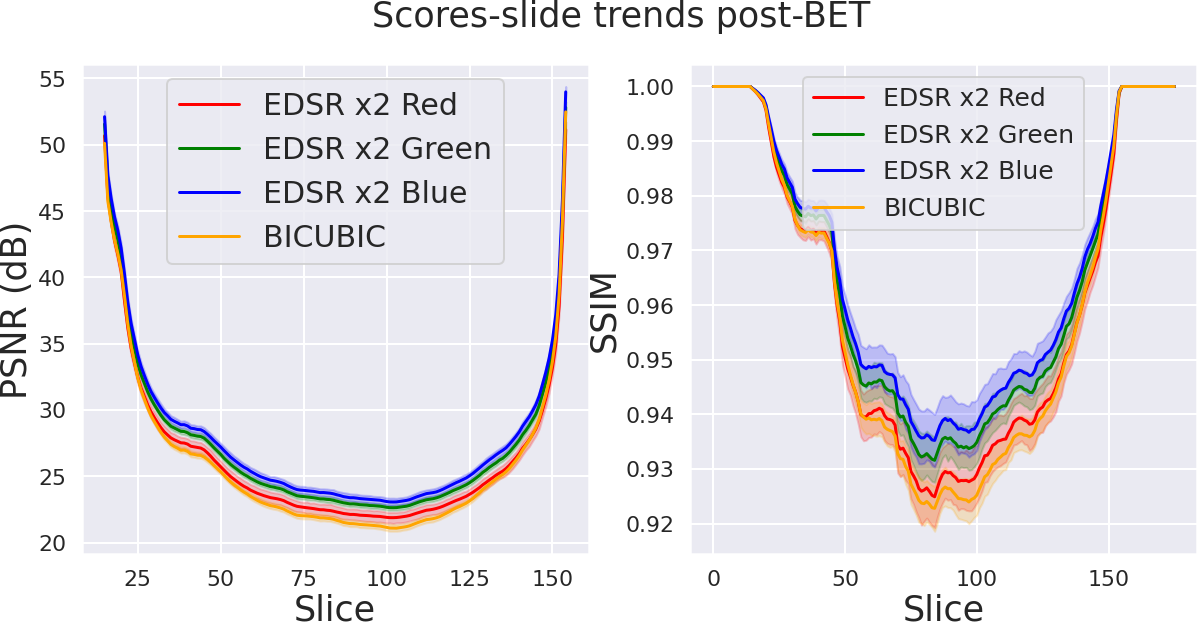
\includegraphics[scale=0.14]{./images/EDSR_score_slide_t1_betted.png}
      \end{figure}
    \end{column}
    
    \begin{column}{0.5\textwidth}
      \begin{itemize}
        \item The same mask is applied to each reconstruction.
        \item Removes background and scalp.
        \item The relative results change:
          \begin{itemize}
            \item channels much more consistent
            \item SR still better than bicubic
          \end{itemize}
      \end{itemize}
    \end{column}
  \end{columns}  
  
\end{frame}


\begin{frame}{Conclusions}
\Large
  \begin{itemize}
   \item Two new libraries were proposed:
   \begin{itemize}
      \item {\bf NumPyNet} Focused on readability and educational purposes;
      \item {\bf Byron} a tool for efficient implementations in CPUs environment;
   \end{itemize}
   \item Promising results for super-resolution on biomedical images
   \item NN can \textbf{generalize} well, applying their ``knowledge'' to new datasets. 
   \item extensions on \textbf{explainability} for DL 
  \end{itemize}
  
\end{frame}


\begin{frame}{Future Developments}
  \large
  Future works may include:
  \begin{itemize}
    \item Extensions of {\it Transfer Learning} with \textbf{training}
    \item Re-train from scratch
    \item Analysis after Brain Extraction for all patients and angles
  \end{itemize}

\end{frame}

\begin{frame}
 \centering
 \huge
 Thanks for your attention
\end{frame}

 
\end{document}
